\lhead{\textbf{Basic Algorithms, Fall 2024 \\ CSCI-UA.0310-001}}
\chead{\Large{\textbf{Homework 12}}}
\def\lc{\left\lceil}   
\def\rc{\right\rceil}
\newtheorem{claim}{Claim}
\newtheorem{property}{Property}
\rhead{\textbf{Instructor: Rotem Oshman\\ Name: Ishan Pranav}}
\runningheadrule
\firstpageheadrule
\cfoot{}
\stepcounter{subsection}
\subsection*{References}
Collaborated with Crystal Huang.
\subsection{Dijkstra}
Show the running of Dijkstra's algorithm for finding the distance from $A$ to all other vertices in the following graph. You should show the updated distances to all the vertices (i.e., the key of the vertex in the priority queue) after each step in the algorithm.

\begin{figure}[h!]
\begin{center}
  \resizebox{!}{!}{  

\tikzset{every picture/.style={line width=0.75pt}} %set default line width to 0.75pt        

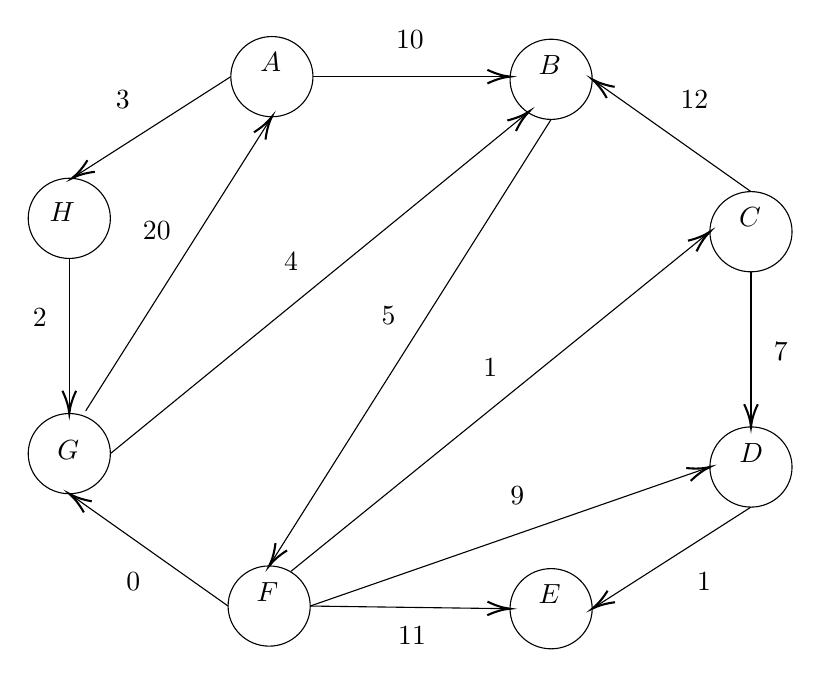
\begin{tikzpicture}[x=0.75pt,y=0.75pt,yscale=-1,xscale=1]
%uncomment if require: \path (0,443); %set diagram left start at 0, and has height of 443

%Shape: Ellipse [id:dp4366659013151436] 
\draw   (193.61,59.32) .. controls (193.61,48.65) and (202.46,40) .. (213.39,40) .. controls (224.32,40) and (233.18,48.65) .. (233.18,59.32) .. controls (233.18,70) and (224.32,78.65) .. (213.39,78.65) .. controls (202.46,78.65) and (193.61,70) .. (193.61,59.32) -- cycle ;
%Shape: Ellipse [id:dp1933565130763586] 
\draw   (328.14,60.61) .. controls (328.14,49.94) and (337,41.29) .. (347.93,41.29) .. controls (358.86,41.29) and (367.71,49.94) .. (367.71,60.61) .. controls (367.71,71.28) and (358.86,79.93) .. (347.93,79.93) .. controls (337,79.93) and (328.14,71.28) .. (328.14,60.61) -- cycle ;
%Shape: Ellipse [id:dp6804484495341399] 
\draw   (424.43,134.04) .. controls (424.43,123.37) and (433.29,114.72) .. (444.22,114.72) .. controls (455.14,114.72) and (464,123.37) .. (464,134.04) .. controls (464,144.71) and (455.14,153.36) .. (444.22,153.36) .. controls (433.29,153.36) and (424.43,144.71) .. (424.43,134.04) -- cycle ;
%Shape: Ellipse [id:dp5474703006205862] 
\draw   (424.43,247.4) .. controls (424.43,236.73) and (433.29,228.08) .. (444.22,228.08) .. controls (455.14,228.08) and (464,236.73) .. (464,247.4) .. controls (464,258.07) and (455.14,266.72) .. (444.22,266.72) .. controls (433.29,266.72) and (424.43,258.07) .. (424.43,247.4) -- cycle ;
%Shape: Ellipse [id:dp8638791225560539] 
\draw   (328.14,315.68) .. controls (328.14,305) and (337,296.35) .. (347.93,296.35) .. controls (358.86,296.35) and (367.71,305) .. (367.71,315.68) .. controls (367.71,326.35) and (358.86,335) .. (347.93,335) .. controls (337,335) and (328.14,326.35) .. (328.14,315.68) -- cycle ;
%Shape: Ellipse [id:dp008449392382588905] 
\draw   (192.29,314.39) .. controls (192.29,303.72) and (201.14,295.07) .. (212.07,295.07) .. controls (223,295.07) and (231.86,303.72) .. (231.86,314.39) .. controls (231.86,325.06) and (223,333.71) .. (212.07,333.71) .. controls (201.14,333.71) and (192.29,325.06) .. (192.29,314.39) -- cycle ;
%Shape: Ellipse [id:dp33826626675219873] 
\draw   (96,240.96) .. controls (96,230.29) and (104.86,221.64) .. (115.78,221.64) .. controls (126.71,221.64) and (135.57,230.29) .. (135.57,240.96) .. controls (135.57,251.63) and (126.71,260.28) .. (115.78,260.28) .. controls (104.86,260.28) and (96,251.63) .. (96,240.96) -- cycle ;
%Shape: Ellipse [id:dp6507975960123465] 
\draw   (96,127.6) .. controls (96,116.93) and (104.86,108.28) .. (115.78,108.28) .. controls (126.71,108.28) and (135.57,116.93) .. (135.57,127.6) .. controls (135.57,138.27) and (126.71,146.92) .. (115.78,146.92) .. controls (104.86,146.92) and (96,138.27) .. (96,127.6) -- cycle ;
%Straight Lines [id:da4219287944911677] 
\draw    (369.35,61.77) -- (444.22,114.72) ;
\draw [shift={(367.71,60.61)}, rotate = 35.27] [color={rgb, 255:red, 0; green, 0; blue, 0 }  ][line width=0.75]    (10.93,-3.29) .. controls (6.95,-1.4) and (3.31,-0.3) .. (0,0) .. controls (3.31,0.3) and (6.95,1.4) .. (10.93,3.29)   ;
%Straight Lines [id:da5980913207552611] 
\draw    (117.42,261.44) -- (192.29,314.39) ;
\draw [shift={(115.78,260.28)}, rotate = 35.27] [color={rgb, 255:red, 0; green, 0; blue, 0 }  ][line width=0.75]    (10.93,-3.29) .. controls (6.95,-1.4) and (3.31,-0.3) .. (0,0) .. controls (3.31,0.3) and (6.95,1.4) .. (10.93,3.29)   ;
%Straight Lines [id:da9818030529391072] 
\draw    (444.22,153.36) -- (444.22,226.08) ;
\draw [shift={(444.22,228.08)}, rotate = 270] [color={rgb, 255:red, 0; green, 0; blue, 0 }  ][line width=0.75]    (10.93,-3.29) .. controls (6.95,-1.4) and (3.31,-0.3) .. (0,0) .. controls (3.31,0.3) and (6.95,1.4) .. (10.93,3.29)   ;
%Straight Lines [id:da8226912095218192] 
\draw    (444.22,266.72) -- (369.4,314.6) ;
\draw [shift={(367.71,315.68)}, rotate = 327.39] [color={rgb, 255:red, 0; green, 0; blue, 0 }  ][line width=0.75]    (10.93,-3.29) .. controls (6.95,-1.4) and (3.31,-0.3) .. (0,0) .. controls (3.31,0.3) and (6.95,1.4) .. (10.93,3.29)   ;
%Straight Lines [id:da9411403626711399] 
\draw    (231.86,314.39) -- (326.14,315.65) ;
\draw [shift={(328.14,315.68)}, rotate = 180.77] [color={rgb, 255:red, 0; green, 0; blue, 0 }  ][line width=0.75]    (10.93,-3.29) .. controls (6.95,-1.4) and (3.31,-0.3) .. (0,0) .. controls (3.31,0.3) and (6.95,1.4) .. (10.93,3.29)   ;
%Straight Lines [id:da04931761460163331] 
\draw    (233.18,59.32) -- (326.14,59.32) ;
\draw [shift={(328.14,59.32)}, rotate = 180] [color={rgb, 255:red, 0; green, 0; blue, 0 }  ][line width=0.75]    (10.93,-3.29) .. controls (6.95,-1.4) and (3.31,-0.3) .. (0,0) .. controls (3.31,0.3) and (6.95,1.4) .. (10.93,3.29)   ;
%Straight Lines [id:da7139612650029891] 
\draw    (115.78,146.92) -- (115.78,219.64) ;
\draw [shift={(115.78,221.64)}, rotate = 270] [color={rgb, 255:red, 0; green, 0; blue, 0 }  ][line width=0.75]    (10.93,-3.29) .. controls (6.95,-1.4) and (3.31,-0.3) .. (0,0) .. controls (3.31,0.3) and (6.95,1.4) .. (10.93,3.29)   ;
%Straight Lines [id:da15021042776281257] 
\draw    (193.61,59.32) -- (118.79,107.2) ;
\draw [shift={(117.1,108.28)}, rotate = 327.39] [color={rgb, 255:red, 0; green, 0; blue, 0 }  ][line width=0.75]    (10.93,-3.29) .. controls (6.95,-1.4) and (3.31,-0.3) .. (0,0) .. controls (3.31,0.3) and (6.95,1.4) .. (10.93,3.29)   ;
%Straight Lines [id:da05554213731104107] 
\draw    (123.7,220.35) -- (212.32,80.34) ;
\draw [shift={(213.39,78.65)}, rotate = 122.33] [color={rgb, 255:red, 0; green, 0; blue, 0 }  ][line width=0.75]    (10.93,-3.29) .. controls (6.95,-1.4) and (3.31,-0.3) .. (0,0) .. controls (3.31,0.3) and (6.95,1.4) .. (10.93,3.29)   ;
%Straight Lines [id:da4376820533976681] 
\draw    (135.57,240.96) -- (335.83,77.34) ;
\draw [shift={(337.38,76.07)}, rotate = 140.75] [color={rgb, 255:red, 0; green, 0; blue, 0 }  ][line width=0.75]    (10.93,-3.29) .. controls (6.95,-1.4) and (3.31,-0.3) .. (0,0) .. controls (3.31,0.3) and (6.95,1.4) .. (10.93,3.29)   ;
%Straight Lines [id:da22701364215684228] 
\draw    (213.14,293.37) -- (347.93,79.93) ;
\draw [shift={(212.07,295.07)}, rotate = 302.27] [color={rgb, 255:red, 0; green, 0; blue, 0 }  ][line width=0.75]    (10.93,-3.29) .. controls (6.95,-1.4) and (3.31,-0.3) .. (0,0) .. controls (3.31,0.3) and (6.95,1.4) .. (10.93,3.29)   ;
%Straight Lines [id:da5780556586002948] 
\draw    (222.62,297.64) -- (422.88,135.3) ;
\draw [shift={(424.43,134.04)}, rotate = 140.97] [color={rgb, 255:red, 0; green, 0; blue, 0 }  ][line width=0.75]    (10.93,-3.29) .. controls (6.95,-1.4) and (3.31,-0.3) .. (0,0) .. controls (3.31,0.3) and (6.95,1.4) .. (10.93,3.29)   ;
%Straight Lines [id:da7820765166034285] 
\draw    (231.86,314.39) -- (422.54,248.06) ;
\draw [shift={(424.43,247.4)}, rotate = 160.82] [color={rgb, 255:red, 0; green, 0; blue, 0 }  ][line width=0.75]    (10.93,-3.29) .. controls (6.95,-1.4) and (3.31,-0.3) .. (0,0) .. controls (3.31,0.3) and (6.95,1.4) .. (10.93,3.29)   ;

% Text Node
\draw (206.55,46.57) node [anchor=north west][inner sep=0.75pt]    {$A$};
% Text Node
\draw (340.61,47.86) node [anchor=north west][inner sep=0.75pt]    {$B$};
% Text Node
\draw (437.22,121.29) node [anchor=north west][inner sep=0.75pt]    {$C$};
% Text Node
\draw (437.37,234.65) node [anchor=north west][inner sep=0.75pt]    {$D$};
% Text Node
\draw (340.61,302.92) node [anchor=north west][inner sep=0.75pt]    {$E$};
% Text Node
\draw (204.75,301.64) node [anchor=north west][inner sep=0.75pt]    {$F$};
% Text Node
\draw (108.78,233.36) node [anchor=north west][inner sep=0.75pt]    {$G$};
% Text Node
\draw (104.99,118.71) node [anchor=north west][inner sep=0.75pt]    {$H$};
% Text Node
\draw (272,36) node [anchor=north west][inner sep=0.75pt]   [align=left] {10};
% Text Node
\draw (137,65) node [anchor=north west][inner sep=0.75pt]   [align=left] {3};
% Text Node
\draw (97,170) node [anchor=north west][inner sep=0.75pt]   [align=left] {2};
% Text Node
\draw (150,128) node [anchor=north west][inner sep=0.75pt]   [align=left] {20};
% Text Node
\draw (218,143) node [anchor=north west][inner sep=0.75pt]   [align=left] {4};
% Text Node
\draw (265,169) node [anchor=north west][inner sep=0.75pt]   [align=left] {5};
% Text Node
\draw (142,297) node [anchor=north west][inner sep=0.75pt]   [align=left] {0};
% Text Node
\draw (314,194) node [anchor=north west][inner sep=0.75pt]   [align=left] {1};
% Text Node
\draw (273,323) node [anchor=north west][inner sep=0.75pt]   [align=left] {11};
% Text Node
\draw (327,255.4) node [anchor=north west][inner sep=0.75pt]    {$9$};
% Text Node
\draw (454,186) node [anchor=north west][inner sep=0.75pt]   [align=left] {7};
% Text Node
\draw (417,297) node [anchor=north west][inner sep=0.75pt]   [align=left] {1};
% Text Node
\draw (409,65) node [anchor=north west][inner sep=0.75pt]   [align=left] {12};


\end{tikzpicture}}
  \end{center}
        \caption{Directed and weighted graph $G$}
    \label{fig:mst}
\end{figure}

For ease of representing your solution, simply complete the following
table. The first row (Step 0) represents the initial values.

\begin{table}[H]
    \centering
\begin{tabular}{|l|c|l|l|l|l|l|l|l|l|}
\hline
Step & \begin{tabular}[c]{@{}c@{}}Vertex Removed\\ from Q\end{tabular} & $A.d$ & $B.d$ & $C.d$ & $D.d$ & $E.d$ & $F.d$ & $G.d$ & $H.d$ \\ \hline
0    &   -   & $0$    &    $\infty$ & $\infty$  & $\infty$    &    $\infty$ & $\infty$    &    $\infty$ & $\infty$    \\ \hline
1    & $A$ & $0$ & $10$ & $\infty$ & $\infty$ & $\infty$ & $\infty$ & $\infty$ & $3$ \\ \hline
2    & $H$ & $0$ & $10$ & $\infty$ & $\infty$ & $\infty$ & $\infty$ & $5$ & $3$ \\ \hline
3    & $G$ & $0$ & $9$ & $\infty$ & $\infty$ & $\infty$ & $\infty$ & $5$ & $3$ \\ \hline
4    & $B$ & $0$ & $9$ & $\infty$ & $\infty$ & $\infty$ & $14$ & $5$ & $3$ \\ \hline
5    & $F$ & $0$ & $9$ & $15$ & $23$ & $25$ & $14$ & $5$ & $3$ \\ \hline
6    & $C$ & $0$ & $9$ & $15$ & $22$ & $25$ & $14$ & $5$ & $3$ \\ \hline
7    & $D$ & $0$ & $9$ & $15$ & $22$ & $23$ & $14$ & $5$ & $3$ \\ \hline
8    & $E$ & $0$ & $9$ & $15$ & $22$ & $23$ & $14$ & $5$ & $3$ \\ \hline
\end{tabular}
    \caption{Execution trace of Dijkstra on $G$.}
    \label{tab:dijkstra}
\end{table}

\begin{solution}
By stepping through Dijkstra's algorithm, we obtain the distances above.
\end{solution}
\subsection{Floyd-Warshall}
Consider again the graph from Question~1. In the following, complete the first four steps of the Floyd-Warshall algorithm by filling four copies of the following table corresponding to $DP[*,*,1]$, $DP[*,*,2]$, $DP[*,*,3]$, and $DP[*,*,4]$. In other words, compute the shortest distances between every pair of vertices when only using nodes $\{A\}$, $\{A,B\}$, $\{A,B,C\}$, and only using $\{A,B,C,D\}$ as intermediate vertices.

\begin{table}[H]
    \centering
\begin{tabular}{|l|l|l|l|l|l|l|l|l|}
\hline
 & $A$ & $B$ & $C$ & $D$ & $E$ & $F$ & $G$ & $H$ \\ \hline
$A$ & & & & & & & & \\ \hline
$B$ & & & & & & & & \\ \hline
$C$ & & & & & & & & \\ \hline
$D$ & & & & & & & & \\ \hline
$E$ & & & & & & & & \\ \hline
$F$ & & & & & & & & \\ \hline
$G$ & & & & & & & & \\ \hline
$H$ & & & & & & & & \\ \hline
\end{tabular}
    \caption{Shortest distance when only using first $i$ vertices as intermediates.}
\end{table}
\begin{solution}
Stepping through the first four iterations of the outer loop of the Floyd--Warshall algorithm gives the results below.
\begin{table}[H]
    \centering
\begin{tabular}{|l|l|l|l|l|l|l|l|l|}
\hline
 & $A$ & $B$ & $C$ & $D$ & $E$ & $F$ & $G$ & $H$ \\ \hline
$A$ & $0$ & $10$ & $\infty$ & $\infty$ & $\infty$ & $\infty$ & $\infty$ & $3$ \\ \hline
$B$    & $\infty$ & $0$ & $\infty$ & $\infty$ & $\infty$ & $5$ & $\infty$ & $\infty$ \\ \hline
$C$    & $\infty$ & $12$ & $0$ & $7$ & $\infty$ & $\infty$ & $\infty$ & $\infty$ \\ \hline
$D$    & $\infty$ & $\infty$ & $\infty$ & $0$ & $1$ & $\infty$ & $\infty$ & $\infty$ \\ \hline
$E$    & $\infty$ & $\infty$ & $\infty$ & $\infty$ & $0$ & $\infty$ & $\infty$ & $\infty$ \\ \hline
$F$    & $\infty$ & $\infty$ & $1$ & $9$ & $11$ & $0$ & $0$ & $\infty$ \\ \hline
$G$    & $20$ & $4$ & $\infty$ & $\infty$ & $\infty$ & $\infty$ & $0$ & $23$ \\ \hline
$H$    & $\infty$ & $\infty$ & $\infty$ & $\infty$ & $\infty$ & $\infty$ & $2$ & $0$ \\ \hline
\end{tabular}
\caption{Shortest distance when only using first $1$ vertex as an intermediate.}
\end{table}
\begin{table}[H]
    \centering
\begin{tabular}{|l|l|l|l|l|l|l|l|l|}
\hline
 & $A$ & $B$ & $C$ & $D$ & $E$ & $F$ & $G$ & $H$ \\ \hline
$A$ & $0$ & $10$ & $\infty$ & $\infty$ & $\infty$ & $15$ & $\infty$ & $3$ \\ \hline
$B$    & $\infty$ & $0$ & $\infty$ & $\infty$ & $\infty$ & $5$ & $\infty$ & $\infty$ \\ \hline
$C$    & $\infty$ & $12$ & $0$ & $7$ & $\infty$ & $17$ & $\infty$ & $\infty$ \\ \hline
$D$    & $\infty$ & $\infty$ & $\infty$ & $0$ & $1$ & $\infty$ & $\infty$ & $\infty$ \\ \hline
$E$    & $\infty$ & $\infty$ & $\infty$ & $\infty$ & $0$ & $\infty$ & $\infty$ & $\infty$ \\ \hline
$F$    & $\infty$ & $\infty$ & $1$ & $9$ & $11$ & $0$ & $0$ & $\infty$ \\ \hline
$G$    & $20$ & $4$ & $\infty$ & $\infty$ & $\infty$ & $9$ & $0$ & $23$ \\ \hline
$H$    & $\infty$ & $\infty$ & $\infty$ & $\infty$ & $\infty$ & $\infty$ & $2$ & $0$ \\ \hline
\end{tabular}
\caption{Shortest distance when only using first $2$ vertices as intermediates.}
\end{table}
\begin{table}[H]
    \centering
\begin{tabular}{|l|l|l|l|l|l|l|l|l|}
\hline
 & $A$ & $B$ & $C$ & $D$ & $E$ & $F$ & $G$ & $H$ \\ \hline
$A$ & $0$ & $10$ & $\infty$ & $\infty$ & $\infty$ & $15$ & $\infty$ & $3$ \\ \hline
$B$    & $\infty$ & $0$ & $\infty$ & $\infty$ & $\infty$ & $5$ & $\infty$ & $\infty$ \\ \hline
$C$    & $\infty$ & $12$ & $0$ & $7$ & $\infty$ & $17$ & $\infty$ & $\infty$ \\ \hline
$D$    & $\infty$ & $\infty$ & $\infty$ & $0$ & $1$ & $\infty$ & $\infty$ & $\infty$ \\ \hline
$E$    & $\infty$ & $\infty$ & $\infty$ & $\infty$ & $0$ & $\infty$ & $\infty$ & $\infty$ \\ \hline
$F$    & $\infty$ & $13$ & $1$ & $8$ & $11$ & $0$ & $0$ & $\infty$ \\ \hline
$G$    & $20$ & $4$ & $\infty$ & $\infty$ & $\infty$ & $9$ & $0$ & $23$ \\ \hline
$H$    & $\infty$ & $\infty$ & $\infty$ & $\infty$ & $\infty$ & $\infty$ & $2$ & $0$ \\ \hline
\end{tabular}
\caption{Shortest distance when only using first $3$ vertices as intermediates.}
\end{table}
\begin{table}[H]
    \centering
\begin{tabular}{|l|l|l|l|l|l|l|l|l|}
\hline
 & $A$ & $B$ & $C$ & $D$ & $E$ & $F$ & $G$ & $H$ \\ \hline
$A$ & $0$ & $10$ & $\infty$ & $\infty$ & $\infty$ & $15$ & $\infty$ & $3$ \\ \hline
$B$    & $\infty$ & $0$ & $\infty$ & $\infty$ & $\infty$ & $5$ & $\infty$ & $\infty$ \\ \hline
$C$    & $\infty$ & $12$ & $0$ & $7$ & $8$ & $17$ & $\infty$ & $\infty$ \\ \hline
$D$    & $\infty$ & $\infty$ & $\infty$ & $0$ & $1$ & $\infty$ & $\infty$ & $\infty$ \\ \hline
$E$    & $\infty$ & $\infty$ & $\infty$ & $\infty$ & $0$ & $\infty$ & $\infty$ & $\infty$ \\ \hline
$F$    & $\infty$ & $13$ & $1$ & $8$ & $9$ & $0$ & $0$ & $\infty$ \\ \hline
$G$    & $20$ & $4$ & $\infty$ & $\infty$ & $\infty$ & $9$ & $0$ & $23$ \\ \hline
$H$    & $\infty$ & $\infty$ & $\infty$ & $\infty$ & $\infty$ & $\infty$ & $2$ & $0$ \\ \hline
\end{tabular}
\caption{Shortest distance when only using first $4$ vertices as intermediates.}
\end{table}
\end{solution}
\newpage
\subsection{Shortest path}
\label{question:birthdayparty}
Sam, who lives in a node $s$ of a weighted \emph{undirected} graph $G = (V, E)$ with non-negative weights, is invited to a birthday party located at a node $h$. Naturally, Sam wants to get from $s$ to $h$ as soon as possible, but they are told to buy some beer on the way over. They can get beer at any supermarket, and the supermarkets form a subset of the vertices $B \subseteq V$. Thus, starting at $s$, they must go to some node $b \in B$ of their choice, and then head from $b$ to $h$ using the shortest total route possible (assume they waste no time in the supermarket). Help Sam to reach $h$ as soon as possible, by solving the following sub-problems. 

\begin{enumerate}
\item Compute the shortest distance from $s$ to all supermarkets $b \in B$.
\begin{solution}
Sam can use Dijkstra's algorithm (denoted {\sc Dijkstra}($G,s$)) to compute the shortest distance from $s$ to all supermarkets $b\in B$.

\textbf{Algorithm I. }{\sc ToSupermarkets}($G,s,B$) requires graph $G=(V,E)$, source vertex $s\in V$, and supermarket vertices $B\subseteq V$.

$(D,P)\leftarrow$ invoke {\sc Dijkstra}($G,s$) for graph $G=(V,E)$ and source vertex $s$; for all $v\in V$, the value at $D[v]$ represents the shortest distance from $s$ to $v$ and $P[v]$ represents the shortest path from $s$ to $v$.

Return $(D,P)$, noting that for all $b\in B$, the value at $D[b]$ represents the shortest distance from $s$ to $b$ and $P[b]$ represents the shortest path from $s$ to $b$.
\end{solution}
\item Compute the shortest distance from every supermarket $b \in B$ to $h$. Note that this is the dual of the single-source shortest path where we are now asking for the shortest path from every node to a particular destination.
\begin{solution}
Again, Sam can use Dijkstra's algorithm to compute the shortest distance from $h$ to all supermarkets $b\in B$, leveraging the fact that $G$ is an undirected graph to reverse the direction of the search without impacting the results.

\textbf{Algorithm II. }{\sc FromSupermarkets}($G,B,h$) requires graph $G=(V,E)$, supermarket vertices $B\subseteq V$, and target vertex $h\in V$.

$(D,P)\leftarrow $ invoke {\sc Dijkstra}($G,h$) for graph $G=(V,E)$ and source vertex $h$; for all $v\in V$, the value at $D[v]$ represents the shortest distance from $h$ to $v$, and $P[v]$ represents the shortest path from $h$ to $v$. Since $G$ is undirected, $D[v]$ also represents the distance from $v$ to $h$, and $P[v]$ also represents the shortest path from $v$ to $h$.

Return $(D,P)$, noting that for all $b\in B$, the value at $D[b]$ represents the shortest distance from $b$ to $h$ and $P[b]$ represents the shortest path from $b$ to $h$.
\end{solution}
\newpage
\item Combine parts 1 and 2 to solve the full problem.
\begin{solution}
Sam should take the shortest overall path; that is, Sam should choose the supermarket $b\in B$ which minimizes the sum of the distances from $s$ to $b$ and $b$ to $h$.

\textbf{Algorithm III. }{\sc ToBirthdayParty}($G,s,B,h$) requires graph $G=(V,E)$, source vertex $s\in V$, supermarket vertices $B\subseteq V$, and target vertex $h\in V$:

Let $b^*\leftarrow\mathsf{nil}$.

Let $d^*\leftarrow+\infty$.

Let $p^*\leftarrow\mathsf{nil}$.

Assign $(D_s,P_s)\leftarrow $ invoke {\sc ToSupermarkets}($G,s,B$).

Assign $(D_h,P_h)\leftarrow $ invoke {\sc FromSupermarkets}($G,B,h$).

For $b\in B$:
\begin{itemize}
\item if $D_s[b]+D_h[b]<d^*$, then:
\begin{itemize}
\item assign $b^*\leftarrow b$;
\item assign $d^*\leftarrow D_s[b]+D_h[b]$;
\item assign $p^*\leftarrow $ concatenation of $P_s[b]$ and $P_h[b]$.
\end{itemize}
\end{itemize}
Return $p^*$, the shortest path from $s$ to $h$ via some $b\in B$.
\end{solution}
\end{enumerate}
\newpage
\subsection{Detecting negative cycles}
A negative weight cycle is a cycle where the sum of the weights of the edges in the cycle is negative. In many algorithms, these negative weight cycles can prove to be problematic, so we want a way to detect them ahead of time. How can we use the output of the Floyd-Warshall algorithm to detect the presence
of a negative-weight cycle in a directed graph?
\begin{solution}

\textbf{Algorithm 1. }{\sc ContainsNegativeCycle}($W,n$) where $W[i,j]$ is the weight of edge $(i,j)$ (or $\infty$ if the edge is absent) and $n$ is the number of vertices; returns $\mathrm{true}$ if the graph represented by $W$ and $n$ contains a negative-weight cycle; otherwise, $\mathrm{false}$:

Let $D\leftarrow\textsc{Floyd--Warshall}(W,n)$.

For $i=1$ to $n$:
\begin{itemize}
    \item if $W[i,i]<0$, then return $\mathrm{true}$.
\end{itemize}

Return $\mathrm{false}$.\\

\textbf{Proposition 1. }\textit{Claim. }Algorithm 1 is correct.

\textit{Proof. }Algorithm 1 returns $\mathrm{true}$ if there is a vertex with a negative self-weight, and $\mathrm{false}$ otherwise. This is correct if the following statement holds: \textit{there is a vertex with a negative self-weight if and only if there is a negative-weight cycle}.
\begin{itemize}
\item Suppose there is a vertex $v$ where, at termination, $W[v,v]<0$. The {\sc Floyd--Warshall} algorithm initializes $W[v,v]$ to $0$, meaning that the current shortest path from $v$ to $v$ is $(v)$ with cost $0$. Since $v$ has a negative self-weight at termination, we know that the algorithm discovered a cheaper path $P=(v,\dots,v)$ with a total cost $c<0$. Of course, $P$ is a negative-weight cycle. Hence, a negative self-weight implies a negative-weight cycle.

\item Suppose there is a cycle $P=(v,\dots,v)$ with a negative total cost $c<0$. Initially, $W[v][v]=0$ via the zero-cost path $(v)$ from $v$ to $v$. However, $P$ provides a cheaper path. Since, at every step of the algorithm, weights are never increased, we know that the self-weight of $v$ at termination is no greater than $c$. That is, $W[v][v]\leq c<0$. Hence, a negative-weight cycle implies a negative self-weight.
\end{itemize}
The above statement holds. Ergo Algorithm 1 is correct.$~\square$
\end{solution}
\newpage
\subsection{Modified Floyd--Warshall}
Consider the following (simplified) pseudocode of the Floyd-Warshall algorithm. $W[i,j]$ is the weight of the edge $i\rightarrow j$ (or $\infty$ if the edge is absent). At the end of the execution of this algorithm, $D[i,j]$ contains the length of the shortest path from $i$ to $j$. First, convince yourself that this is indeed the case (no need to submit this part).

\begin{code}
	{\sc Floyd-Warshall}$(W,n)$\\
	1 \> \For $i=1$ \To $n$\\
	2 \> \> \For $j=1$ \To $n$\\
	3 \> \> \> $D[i,j]=W[i,j]$\\
	4 \> \For $k=1$ \To $n$\\
	5 \> \> \For $i=1$ \To $n$\\
	6 \> \> \> \For $j=1$ \To $n$\\
	7 \> \> \> \> $cost=D[i,k]+D[k,j]$\\
	8 \> \> \> \> \If $cost<D[i,j]$ \\
	9 \> \> \> \> \> $D[i,j]=cost$\\
\end{code}
Now, consider the modification where, instead of at line 4 above, the iterator for $k$ is nested within the loop for the variable $j$, i.e.:
\begin{code}
	{\sc Floyd-Warshall-Modified}$(W,n)$\\
	1 \> \For $i=1$ \To $n$\\
	2 \> \> \For $j=1$ \To $n$\\
	3 \> \> \> $D[i,j]=W[i,j]$\\
	4 \> \For $i=1$ \To $n$\\
	5 \> \> \For $j=1$ \To $n$\\
	6 \> \> \> \For $k=1$ \To $n$\\
	7 \> \> \> \> $cost=D[i,k]+D[k,j]$\\
	8 \> \> \> \> \If $cost<D[i,j]$ \\
	9 \> \> \> \> \> $D[i,j]=cost$\\
\end{code}
What is the meaning of the value stored at $D[1,2]$, at the end of the execution of this modified algorithm? Justify your answer. 
\begin{solution}
At the end of the execution of this modified algorithm, the value stored at $D[1,2]$ is the shortest distance from vertex $i=1$ to vertex $j=2$ via at most $1$ intermediate vertex. In other words, it is the shortest distance from vertex $1$ to vertex $2$ via a direct edge $(1,2)$ or a path $(1,k,2)$ for some other vertex $k$. We can confirm this by stepping through the algorithm.

\textit{First.} The algorithm assigns the shortest distance from $i$ to $j$ to be $W[i,j]$: the weight of the edge $(i,j)$, if it exists, or $+\infty$ if not.

\textit{Second. }The second loop considers $i=1,j=1$. Note that {\sc Floyd-Warshall} is only valid for $W[i,j]\geq 0$, so any path $(1,\dots,1)$ is no cheaper than the direct edge $(1,1)$. So the distance $D[1,1]$ remains $0$.

\textit{Third. }The second loop considers $i=1,j=2$. For each $1\leq k\leq n$, if the path $(i,k,j)$ has a shorter total cost than the existing $D[1,2]$, it is taken. Otherwise, it is not, and $D[1,2]=W[1,2]$. In other words, if there is a path via $1$ intermediate vertex that is cheaper than the existing path via $0$ intermediate vertices, it is taken.

\textit{Thereafter. }The second loop all successive pairs $(i,j)$ after $(1,2)$. If any value in $D$ is ever modified, it is always position $D[i,j]$ for the current pair $(i,j)$. Since for all successive pairs $i>1$ or $j>2$, we know that $D[1,2]$ is not modified during this process.

Hence, the value stored at $D[1,2]$ is either $W[1,2]$ or the shortest distance from $1$ to $2$ via $1$ other vertex, whichever is smaller.
\end{solution}
